\section{Dijkstra Algorithm}

\begin{frame}{Dijkstra Algorithm}{Shortest Path without Computer}
  \begin{itemize}
    \item
      Wanted: Shortest path from M to all other points
    \item
      Place pearls on crossings and clamp strings between them
  \end{itemize}
  \begin{figure}
    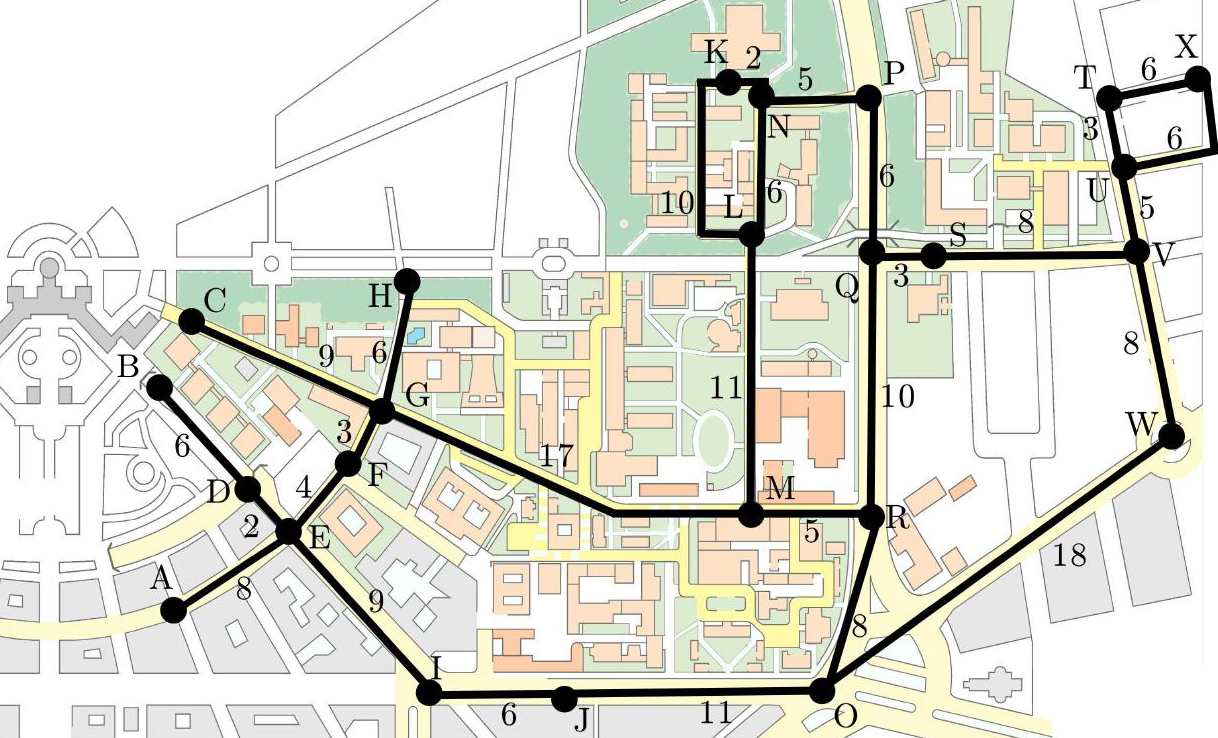
\includegraphics[width=0.75\linewidth]{Images/Dijkstra/DijkstraMap}
    \caption{Map $\copyright\,$ Mehlhorn / Sanders}
  \end{figure}
\end{frame}

%-------------------------------------------------------------------------------

\begin{frame}{Dijkstra Algorithm}{Shortest Path without Computer}
  \vspace{-1.5em}
  \begin{columns}
    \begin{column}{0.55\linewidth}
      \begin{figure}[!t]
        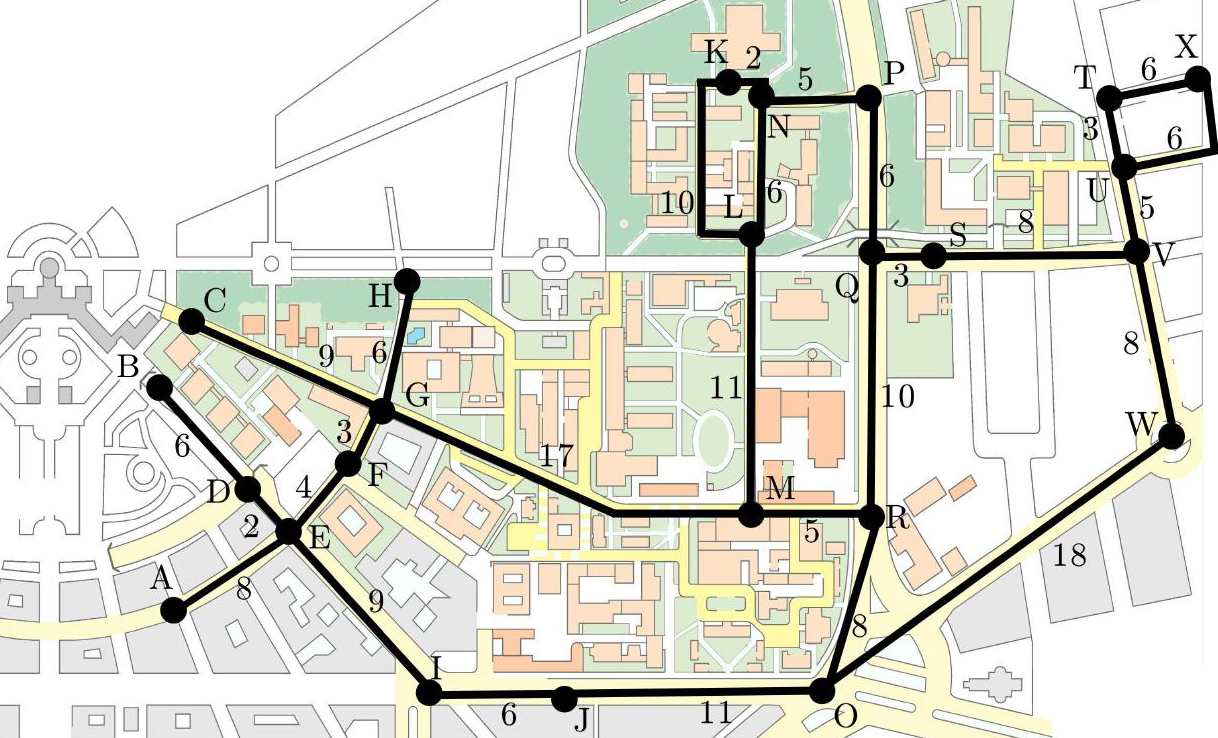
\includegraphics[width=0.8\linewidth]
          {Images/Dijkstra/DijkstraMap}
        \caption{Map $\copyright\,$ Mehlhorn / Sanders}
      \end{figure}
      \vspace{-1.5em}
      \begin{itemize}
        \item
          Take the net and pull it slowly upwards until fully lifted
        \item
          Each node (pearl) now has a specific height
        \item
          The distance to M is exactly the {\color{Mittel-Blau}shortest path}
      \end{itemize}
    \end{column}
    \begin{column}{0.45\linewidth}
      \begin{figure}[!t]
        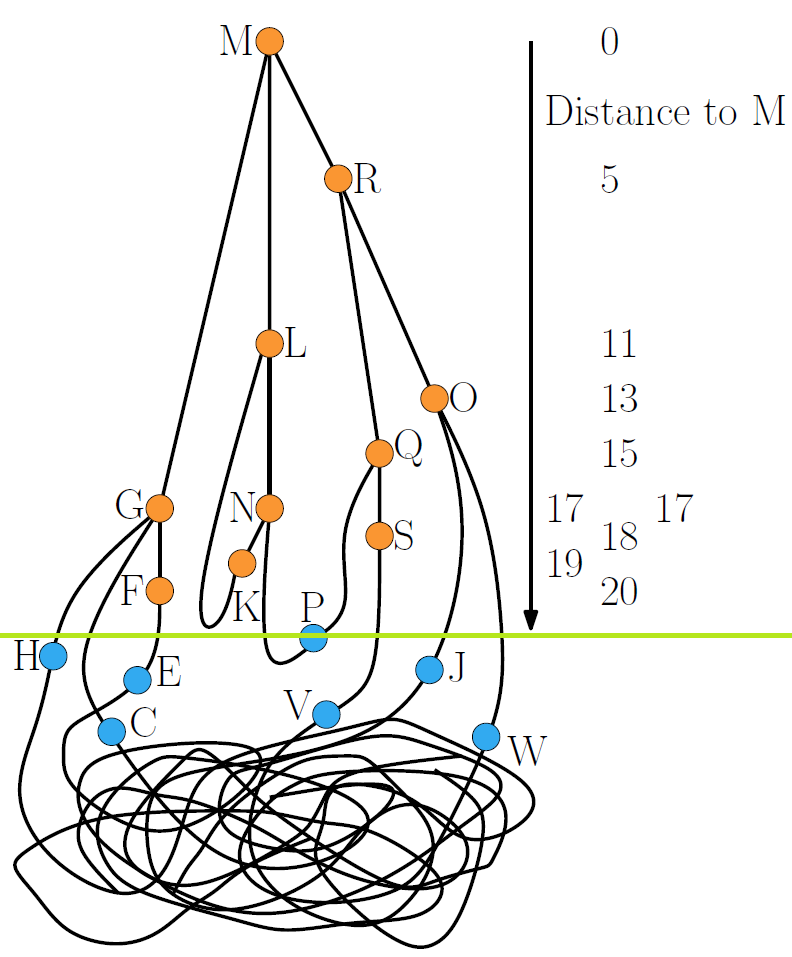
\includegraphics[width=\linewidth]
          {Images/Dijkstra/DijkstraTree_WithOverlay}
        \vspace{-0.5em}
        \caption{Map $\copyright\,$ Mehlhorn / Sanders}
      \end{figure}
    \end{column}
  \end{columns}
\end{frame}

%-------------------------------------------------------------------------------

\begin{frame}{Dijkstra Algorithm}{Shortest Path}
  \vspace{-1.5em}
  \begin{figure}
    \begin{adjustbox}{width=0.75\linewidth}
      \begin{tikzpicture}[
  vertex/.style={
    circle,
    draw=Mittel-Blau,
    color=Mittel-Blau,
    fill=Hell-Blau,
    inner sep=0em,
    minimum size=1.75em,
    line width=0.1em,
    font=\large,
    solid
  }, vertex_shadow/.style={
    vertex,
    draw=black,
    color=black,
    fill=white,
    dotted
  }, edge/.style={
    draw=Mittel-Gruen,
    line width=0.2em
  }, edge_arrow/.style={
    edge,
    ->
  }, edge_label/.style={
    sloped,
    anchor=south,
    auto=false
  }
]%
% Draw vertices
\draw (9.0, 0.0) node[vertex] (end) {$t$};
\draw[edge_arrow, dashdotted]
  (0.0, 0.0) .. controls (3.0, 1.5) and (6.0, 0.0) .. (end.west)
  node[vertex, pos=0.0] {$s$}
  node[vertex, pos=0.2] {$u_1$}
  node[vertex_shadow, pos=0.4] {}
  node[vertex, pos=0.6] {$u_2$}
  node[vertex_shadow, pos=0.8] {}
  node[pos=0.5, above] {\color{Mittel-Gruen}$r$};
\end{tikzpicture}%
    \end{adjustbox}
    \label{fig:dijkstra:shortest_path_introduction}
    \caption{Shortest path from {\color{Mittel-Blau}$s$} to
    {\color{Mittel-Blau}$t$}}
  \end{figure}
  \vspace{-1.5em}
  \begin{itemize}
    \item
      Let {\color{Mittel-Gruen}$r$} be the shortest path from
      {\color{Mittel-Blau}$s$} to {\color{Mittel-Blau}$t$}
    \item
      For each node {\color{Mittel-Blau}$u$} on path {\color{Mittel-Gruen}$r$}
      the path from {\color{Mittel-Blau}$u$} to {\color{Mittel-Blau}$t$} is
      the shortest path
  \end{itemize}
  \textbf{Proof:}
  \begin{itemize}
    \item
      If there was a shorter path from {\color{Mittel-Blau}$s$} to
      {\color{Mittel-Blau}$u$} then we could choose this path to get faster to
      {\color{Mittel-Blau}$t$}
    \item
      Then {\color{Mittel-Gruen}$r$} would not be the shortest path
  \end{itemize}
\end{frame}

%-------------------------------------------------------------------------------

\begin{frame}{Dijkstra Algorithm}{Shortest Path}
  \vspace{-1.5em}
  \begin{figure}
    \begin{adjustbox}{width=0.75\linewidth}
      \begin{tikzpicture}[
  vertex/.style={
    circle,
    draw=Mittel-Blau,
    color=Mittel-Blau,
    fill=Hell-Blau,
    inner sep=0em,
    minimum size=1.75em,
    line width=0.1em,
    font=\large,
    solid
  }, vertex_shadow/.style={
    vertex,
    draw=black,
    color=black,
    fill=white,
    dotted
  }, edge/.style={
    draw=Mittel-Gruen,
    line width=0.2em
  }, edge_arrow/.style={
    edge,
    ->
  }, edge_label/.style={
    sloped,
    anchor=south,
    auto=false
  }
]%
% Draw vertices
\draw (9.0, 0.0) node[vertex] (end) {$t$};
\draw[edge_arrow, dashdotted]
  (0.0, 0.0) .. controls (3.0, 1.5) and (6.0, 0.0) .. (end.west)
  node[vertex, pos=0.0] {$s$}
  node[vertex, pos=0.2] {$u_1$}
  node[vertex_shadow, pos=0.4] {}
  node[vertex, pos=0.6] {$u_2$}
  node[vertex_shadow, pos=0.8] {}
  node[pos=0.5, above] {\color{Mittel-Gruen}$r$};
\end{tikzpicture}%
    \end{adjustbox}
    \label{fig:dijkstra:shortest_path_introduction_re}
    \caption{Shortest path from {\color{Mittel-Blau}$s$} to
      {\color{Mittel-Blau}$t$}}
  \end{figure}
  \vspace{-1.5em}
  \begin{itemize}
    \item
      Let {\color{Mittel-Gruen}$r$} be the shortest path from
      {\color{Mittel-Blau}$s$} to {\color{Mittel-Blau}$t$}
    \item
      For each node {\color{Mittel-Blau}$u$} on path {\color{Mittel-Gruen}$r$}
      the path from {\color{Mittel-Blau}$u$} to {\color{Mittel-Blau}$t$} is
      the shortest path
    \item
      This is also correct for all sub paths on {\color{Mittel-Gruen}$r$}
    \item
      If the shortest path from {\color{Mittel-Blau}$s$} to
      {\color{Mittel-Blau}$t$} passes {\color{Mittel-Blau}$u_1$} and
      {\color{Mittel-Blau}$u_2$} then the sub path
      $({\color{Mittel-Blau}u_1}, {\color{Mittel-Blau}u_2})$
      is the shortest path from {\color{Mittel-Blau}$u_1$} to
      {\color{Mittel-Blau}$u_2$}
  \end{itemize}
\end{frame}

%-------------------------------------------------------------------------------

\begin{frame}{Dijkstra Algorithm}{Shortest Path}
  \begin{figure}%
    \begin{adjustbox}{width=0.75\linewidth}%
      \begin{tikzpicture}[
  vertex/.style={
    circle,
    draw=Mittel-Blau,
    color=Mittel-Blau,
    fill=Hell-Blau,
    inner sep=0em,
    minimum size=1.75em,
    line width=0.1em,
    font=\large,
    solid
  }, vertex_shadow/.style={
    vertex,
    draw=black,
    color=black,
    fill=white,
    dotted
  }, edge/.style={
    draw=Mittel-Gruen,
    line width=0.2em
  }, edge_arrow/.style={
    edge,
    ->
  }, edge_label/.style={
    sloped,
    midway,
    color=Mittel-Gruen
  }
]%
% Draw vertices
\draw (-2.0, 0.0) node[vertex] (start) {$s$};
\draw (10.0, 0.0) node[vertex] (end) {$t$};

\draw[edge_arrow] (7.5, 1.5) node[vertex] (v1) {$v_1$} to
  node[edge_label, above] {16} (end);
\draw[edge_arrow] (7.5, 0.0) node[vertex] (v2) {$v_2$} to
  node[edge_label, above] {3} (end);
\draw[edge_arrow] (7.5, -1.5) node[vertex] (v3) {$v_3$} to
  node[edge_label, above] {2} (end);

\draw[edge_arrow, dashdotted]
  (start) .. controls (3.0, 2.5) and (6.0, 1.0) .. (v1.west)
  node[vertex_shadow, pos=0.2] {}
  node[vertex_shadow, pos=0.4] {}
  node[vertex_shadow, pos=0.6] {}
  node[vertex_shadow, pos=0.8] {}
  node[edge_label, pos=0.5, above] {22};
\draw[edge_arrow, dashdotted]
  (start) .. controls (3.0, -1.0) and (6.0, 0.0) .. (v2.west)
  node[vertex_shadow, pos=0.25] {}
  node[vertex_shadow, pos=0.4] {}
  node[vertex_shadow, pos=0.6] {}
  node[edge_label, pos=0.5, above] {34};
\draw[edge_arrow, dashdotted]
  (start) .. controls (3.0, -3.0) and (6.0, -1.5) .. (v3.west)
  node[vertex_shadow, pos=0.1] {}
  node[vertex_shadow, pos=0.3] {}
  node[vertex_shadow, pos=0.8] {}
  node[edge_label, pos=0.5, above] {42};
\end{tikzpicture}%%
    \end{adjustbox}%
    \vspace{-1.0em}
    \label{fig:dijkstra:shortest_paths_introduction}%
    \caption{Shortest paths from {\color{Mittel-Blau}$s$} to
      {\color{Mittel-Blau}$t$}}
  \end{figure}
  \vspace{-1.0em}
  \begin{itemize}
    \item
      If we know the shortest path form {\color{Mittel-Blau}$s$}
      to the preceding nodes of {\color{Mittel-Blau}$t$}
      \begin{math}
        (
          {\color{Mittel-Blau}v_1},
          {\color{Mittel-Blau}v_2},
          {\color{Mittel-Blau}v_3}
        )
       \end{math}
       we can determine the shortest path to {\color{Mittel-Blau}$t$}
   \end{itemize}
\end{frame}

%-------------------------------------------------------------------------------

\begin{frame}{Dijkstra Algorithm}{Shortest Path}
  \textbf{Idea:}
  \begin{itemize}
    \item
      Attach the cost of the shortest path to each node
    \item
      Let the information travel over the edges (message passing)
    \item
      In which order should we process the nodes?
  \end{itemize}
\end{frame}

%-------------------------------------------------------------------------------

\begin{frame}{Dijkstra Algorithm}
  \begin{columns}
    \begin{column}{0.6\linewidth}
      \textbf{Inventor:}
      \begin{itemize}
        \item
          Edsger Dijkstra (1930 - 2002)
        \item
          Computer scientist from Netherlands
        \item
          Won Turing-Award as one of few Europeans for his studies of 
          structured programming
        \item
          Invented the Dijkstra-Algorithm in 1959
      \end{itemize}
    \end{column}
    \begin{column}{0.4\linewidth}
      \begin{figure}
        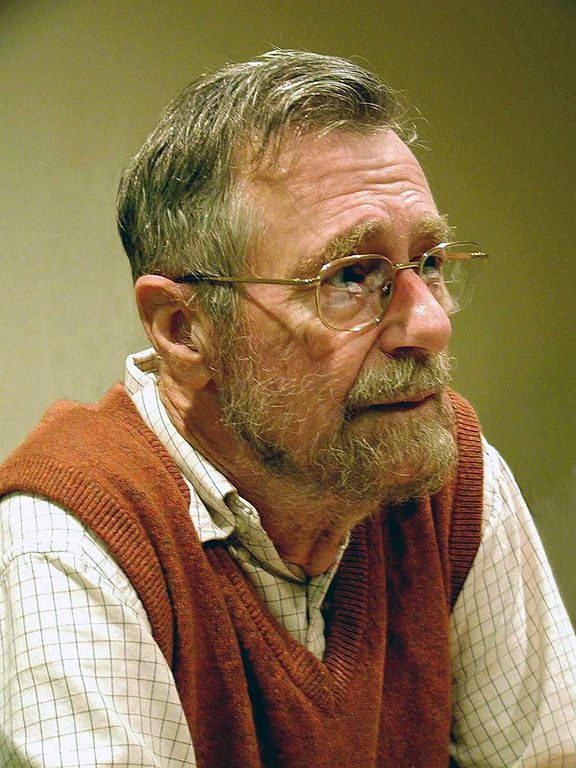
\includegraphics[width=0.75\linewidth]
          {Images/Dijkstra/Edsger_Wybe_Dijkstra.jpg}
        \caption{Portrait \copyright\; Hamilton Richards - manuscripts of
          Edsger W. Dijkstra, University Texas at Austin}
        \label{fig:dijkstra:portrait}
      \end{figure}
    \end{column}
  \end{columns}
\end{frame}

%-------------------------------------------------------------------------------

\begin{frame}{Dijkstra Algorithm}
  \vspace{-1.5em}
  \begin{columns}
    \begin{column}{0.55\linewidth}
      \textbf{Example:}
      \begin{itemize}
        \item
          Lift pearl {\color{Mittel-Blau}$M$} a little bit
        \item
          Connections to pearls {\color{Mittel-Blau}$R$},
          {\color{Mittel-Blau}$L$} and {\color{Mittel-Blau}$G$} are hanging in
          the air
        \item
          Lift further until pearl {\color{Mittel-Blau}$R$} starts to lift at
          $\SI{5}{m}$
        \item
          The shortest path to {\color{Mittel-Blau}$R$} is now known
        \item
          Lift further: The wires from {\color{Mittel-Blau}$R$},
          {\color{Mittel-Blau}$O$} and {\color{Mittel-Blau}$Q$} are now in the
          air
        \item
          One of the pearls {\color{Mittel-Blau}$G$}, {\color{Mittel-Blau}$L$},
          {\color{Mittel-Blau}$Q$} or {\color{Mittel-Blau}$O$} is the next one\\
          {\color{gray}Which one?}
      \end{itemize}
    \end{column}
    \begin{column}{0.45\linewidth}
      \begin{figure}[!t]
        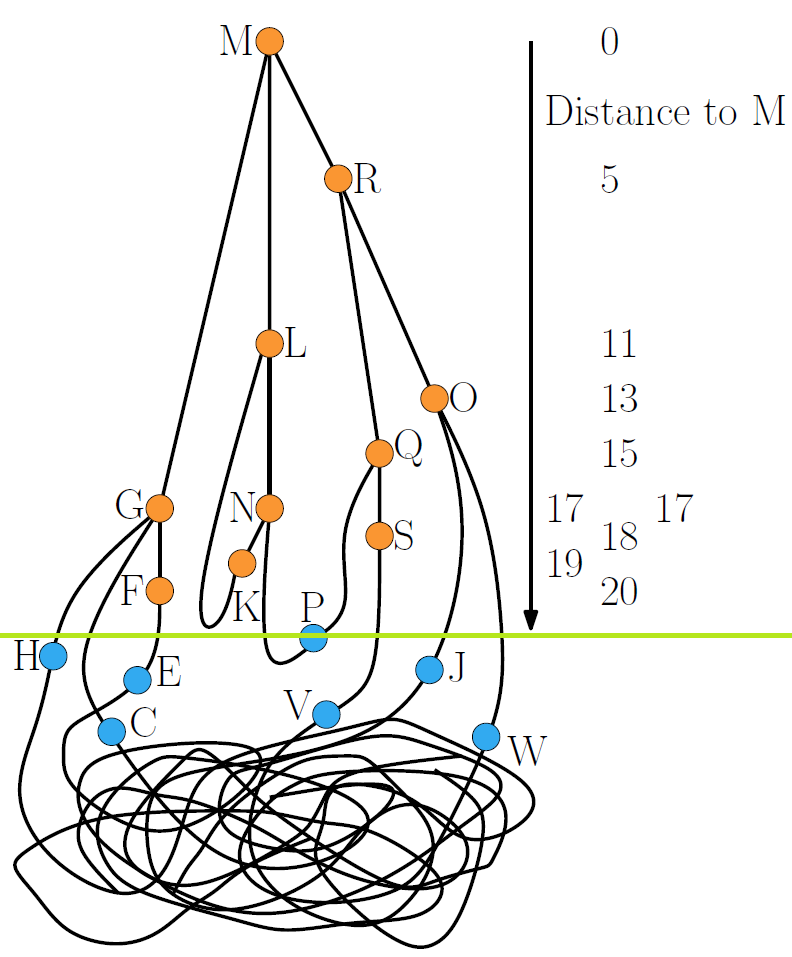
\includegraphics[width=\linewidth]
          {Images/Dijkstra/DijkstraTree_WithOverlay}
        \vspace{-0.5em}
        \caption{Map $\copyright\,$ Mehlhorn / Sanders}
      \end{figure}
    \end{column}
  \end{columns}
\end{frame}

%-------------------------------------------------------------------------------

\begin{frame}{Dijkstra Algorithm}
  \vspace{-1.5em}
  \begin{columns}
    \begin{column}{0.55\linewidth}
      \textbf{Example:}
      \begin{itemize}
        \item
          At $\SI{11}{m}$ pearl {\color{Mittel-Blau}$L$} gets lifted
        \item
          The wires to {\color{Mittel-Blau}$N$} and {\color{Mittel-Blau}$K$}
          are now in the air
        \item
          One of the pearls {\color{Mittel-Blau}$G$}, {\color{Mittel-Blau}$K$},
          {\color{Mittel-Blau}$N$}, {\color{Mittel-Blau}$Q$} or
          {\color{Mittel-Blau}$O$} is the next one\\
          {\color{gray}Which one?}
        \item
          At $\SI{13}{m}$ pearl {\color{Mittel-Blau}$O$} gets lifted\\
          $\cdots$
        \item
          {\color{gray}How to translate this into an computer algorithm?}
      \end{itemize}
    \end{column}
    \begin{column}{0.45\linewidth}
      \begin{figure}[!t]
        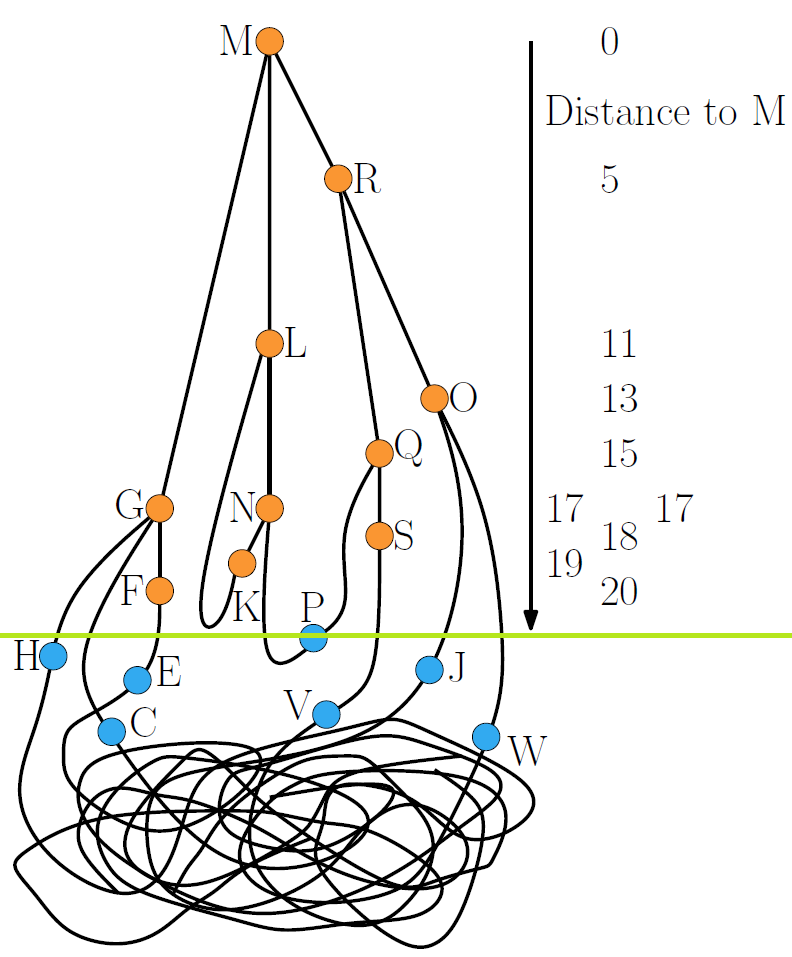
\includegraphics[width=\linewidth]
        {Images/Dijkstra/DijkstraTree_WithOverlay}
        \vspace{-0.5em}
        \caption{Map $\copyright\,$ Mehlhorn / Sanders}
      \end{figure}
    \end{column}
  \end{columns}
\end{frame}

%-------------------------------------------------------------------------------

\begin{frame}{Dijkstra Algorithm}
  \textbf{High level description:}
  Three types of nodes
  \begin{itemize}
    \item
      {\color{Mittel-Blau}Settled:}
      For node {\color{Mittel-Blau}$u$} we know
      {\color{Mittel-Blau}$\mathrm{dist}(s, u)$}
      \hfill
      \raisebox{-0.5em}{\begin{adjustbox}{height=1.5em}%
        \begin{tikzpicture}[
  vertex_base/.style={
    circle,
    inner sep=0em,
    minimum size=1.75em,
    line width=0.1em,
    font=\large,
    solid
  },
  vertex_settled/.style={
    vertex_base,
    draw=Mittel-Blau,
    color=Mittel-Blau,
    fill=orange!50!yellow
  }
]%
\draw (0, 0) node[vertex_settled] {42};
\end{tikzpicture}%
%
      \end{adjustbox}}\\
      {\color{gray}(Pearl example: This preal is hanging in the air)}
      \vspace{0.5em}
    \item
      {\color{Mittel-Blau}Active:}
      For node {\color{Mittel-Blau}$u$} we know a tentative distance
      {\color{Mittel-Blau}$\mathrm{td}(u) \geq \mathrm{dist}(s, u)$}
      (Can be optimal but doesn't have to)
      \hfill
      \raisebox{-0.5em}{\begin{adjustbox}{height=1.5em}%
        \begin{tikzpicture}[
  vertex_base/.style={
    circle,
    inner sep=0em,
    minimum size=1.75em,
    line width=0.1em,
    font=\large,
    solid
  },
  vertex_active/.style={
    vertex_base,
    draw=Mittel-Blau,
    color=Mittel-Blau,
    fill=Hell-Blau
  }
]%
\draw (0, 0) node[vertex_active] {37};
\end{tikzpicture}%
%
      \end{adjustbox}}\\
      {\color{gray}(Pearl example: This pearl is laying on the table but\\
        one connected wire is already in the air)}
        \vspace{0.5em}
    \item
      {\color{Mittel-Blau}Unreached:}
      We have not reached the node yet
      \hfill
      \raisebox{-0.5em}{\begin{adjustbox}{height=1.5em}%
          \begin{tikzpicture}[
  vertex_base/.style={
    circle,
    inner sep=0em,
    minimum size=1.75em,
    line width=0.1em,
    font=\large,
    solid
  }, vertex_unreached/.style={
    vertex_base,
    draw=Mittel-Blau,
    color=Mittel-Blau,
    fill=white
  }
]%
\draw (0, 0) node[vertex_unreached] {};
\end{tikzpicture}%%
        \end{adjustbox}}\\
        {\color{gray}(Pearl example: This preal is hanging in the air)}
  \end{itemize}
\end{frame}

%-------------------------------------------------------------------------------

\begin{frame}{Dijkstra Algorithm}
  \textbf{High level description:}
  \begin{itemize}
    \item
      Each iteration take the {\color{Mittel-Blau}active} node
      {\color{Mittel-Blau}$u$} with the
      {\color{Mittel-Blau}smallest $\mathrm{td}(u)$}\\
      {\color{gray}(The pearl getting lifted next)}
    \item
      We update the state of the node {\color{Mittel-Blau}$u$} to
      {\color{Mittel-Blau}settled}\\
      {\color{gray}(The pearl gets lifted)}
    \item
      We check for each {\color{Mittel-Blau}neighbor $v$} of node
      {\color{Mittel-Blau}$u$} if we can reach {\color{Mittel-Blau}$v$} faster
      than currently possible\\
      {\color{gray}(Check all outgoing wires from this pearl:
        Activate all connected pearls, update
        tentative distance if smaller)}
    \item
      Iterate until no active nodes exist anymore
  \end{itemize}
\end{frame}

%-------------------------------------------------------------------------------

\begin{frame}{Dijkstra Algorithm}
  \vspace{-1em}
  \begin{figure}[!h]
    \begin{adjustbox}{width=\linewidth}
      \begin{tikzpicture}[
  vertex_base/.style={
   circle,
   inner sep=0em,
   minimum size=1.75em,
   line width=0.1em,
   font=\large,
   solid
  }, vertex_active/.style={
    vertex_base,
    draw=Mittel-Blau,
    color=Mittel-Blau,
    fill=Hell-Blau
  }, vertex_settled/.style={
    vertex_base,
    draw=Mittel-Blau,
    color=Mittel-Blau,
    fill=orange!50!yellow
  }, vertex_unreached/.style={
    vertex_base,
    draw=Mittel-Blau,
    color=Mittel-Blau,
    fill=white
  }, vertex_label/.style={
    font=\large,
    color=Mittel-Blau
  }, vertex_old/.style={
    draw,
    color=gray,
    strike out,
    line width=0.1em
  }, edge/.style={
    draw=Mittel-Gruen,
    line width=0.2em
  }, edge_arrow/.style={
    edge,
    ->
  }, edge_cost/.style={
    midway,
    color=Hell-Gruen,
    font=\Large
  }, edge_highlight/.style={
    edge_arrow,
    preaction={
      draw,yellow,-,% Draw yellow without any arrow head
      double=yellow,
      double distance=2\pgflinewidth,
    }
  }, edge_final_highlight/.style={
    edge_arrow,
    preaction={
      draw,red!40!white,-,% Draw yellow without any arrow head
      double=red!40!white,
      double distance=2\pgflinewidth,
    }
  }, reverse/.style={
    ->,
    color=red!90!black,
    line width=0.2em
  }
]%

% Vertex 3 old values
\only<3>{ % Value 1
  \draw ($(4, 0) + (-1em, -1em)$) node[vertex_old] {5};
}
\only<4>{ % Value 2
  \draw ($(4, 0) + (-1em, -1em)$) node[vertex_old] {4};
}

% Vertex 4 old values
\only<5>{ % Value 1
  \draw ($(4, -2.5) + (-1em, -1em)$) node[vertex_old] {10};
}

% Vertex 0
\only<1>{
  \draw (-1.0, 0.0) node[
    vertex_active,
    label={[vertex_label, shift={(-1em, -0.5em)}]above:$u_1$}
  ] (vert0) {0};
}
\only<2->{
  \draw (-1.0, 0.0) node[
    vertex_settled,
    label={[vertex_label, shift={(-1em, -0.5em)}]above:$u_1$}
  ] (vert0) {0};
}

% Vertex 1
\only<1>{
  \draw (2.5, 2.5) node[vertex_unreached] (vert1) {$u_2$};
}
\only<2>{
  \draw (2.5, 2.5) node[
    vertex_active,
    label={[vertex_label, shift={(-1em, -0.5em)}]above:$u_2$}
  ] (vert1) {1};
}
\only<3->{
  \draw (2.5, 2.5) node[
    vertex_settled,
    label={[vertex_label, shift={(-1em, -0.5em)}]above:$u_2$}
  ] (vert1) {1};
}

% Vertex 2 (labels for u5 and u3 are swapped)
\only<1>{
  \draw (4.0, -2.5) node[vertex_unreached] (vert2) {$u_5$};
}
\only<2-5>{
  \draw (4.0, -2.5) node[
    vertex_active,
    label={[vertex_label, shift={(-1.5em, 0em)}]above:$u_5$}
  ] (vert2) {%
    \only<2-4>{10}%
    \only<5->{6}%
  };
}
\only<6->{
  \draw (4.0, -2.5) node[
    vertex_settled,
    label={[vertex_label, shift={(-1.5em, 0em)}]above:$u_5$}
  ] (vert2) {6};
};

% Vertex 3
\only<1>{
  \draw (4.0, 0.0) node[vertex_unreached] (vert3) {$u_4$};
}
\only<2-4>{
  \draw (4.0, 0.0) node[
    vertex_active,
    label={[vertex_label, shift={(-2em, -0.5em)}]$u_4$}
  ] (vert3) {%
    \only<2>{5}%
    \only<3>{4}%
    \only<4>{3}%
  };
}
\only<5->{
  \draw (4.0, 0.0) node[
    vertex_settled,
    label={[vertex_label, shift={(-2em, -0.5em)}]$u_4$}
  ] (vert3) {3};
}

% Vertex 4 (labels for u5 and u3 are swapped)
\only<1-2>{
  \draw (5.5, 2.5) node[vertex_unreached] (vert4) {$u_3$};
}
\only<3>{
  \draw (5.5, 2.5) node[
    vertex_active,
    label={[vertex_label, shift={(1em, -0.5em)}]$u_3$}
  ] (vert4) {2};
}
\only<4->{
  \draw (5.5, 2.5) node[
    vertex_settled,
    label={[vertex_label, shift={(1em, -0.5em)}]$u_3$}
  ] (vert4) {2};
}

% Vertex 5
\only<1-3>{
  \draw (9.0, 0.0) node[vertex_unreached] (vert5) {$u_6$};
}
\only<4-6>{
  \draw (9.0, 0.0) node[
    vertex_active,
    label={[vertex_label, shift={(1em, -0.5em)}]$u_6$}
  ] (vert5) {6};
}
\only<7>{
  \draw (9.0, 0.0) node[
    vertex_settled,
    label={[vertex_label, shift={(1em, -0.5em)}]$u_6$}
  ] (vert5) {6};
}

% Edges from vertex 0
\only<2>{\draw[edge_highlight] (vert0) to node[edge_cost, above] {1} (vert1);}
% Check if highlighting final shortest path
\ifnum \DijkstraReverse>0
  \only<1,3-6>{\draw[edge_arrow] (vert0) to node[edge_cost, above] {1} (vert1);}
  \only<7>{\draw[edge_final_highlight]%
    (vert0) to node[edge_cost, above] {1} (vert1);}
\else
  \only<1,3->{\draw[edge_arrow] (vert0) to node[edge_cost, above] {1} (vert1);}
\fi

\only<1,3->{\draw[edge_arrow] (vert0) to node[edge_cost, above] {10} (vert2);}
\only<2>{\draw[edge_highlight] (vert0) to node[edge_cost, above] {10} (vert2);}

\only<1,3->{\draw[edge_arrow] (vert0) to node[edge_cost, above] {5} (vert3);}
\only<2>{\draw[edge_highlight] (vert0) to node[edge_cost, above] {5} (vert3);}

% Edges from vertex 1
\only<1-2,4->{\draw[edge_arrow] (vert1) to node[edge_cost, above] {3} (vert3);}
\only<3>{\draw[edge_highlight] (vert1) to node[edge_cost, above] {3} (vert3);}

\only<3>{\draw[edge_highlight] (vert1) to node[edge_cost, above] {1} (vert4);}
% Check if highlighting final shortest path
\ifnum \DijkstraReverse>0
  \only<1-2,4-6>{\draw[edge_arrow]%
    (vert1) to node[edge_cost, above] {1} (vert4);}
  \only<7>{\draw[edge_final_highlight]%
    (vert1) to node[edge_cost, above] {1} (vert4);}
\else
  \only<1-2,4->{\draw[edge_arrow]%
    (vert1) to node[edge_cost, above] {1} (vert4);}
\fi

% Edges from vertex 2
\only<1-5,7>{\draw[edge_arrow] (vert2) to node[edge_cost, above] {7} (vert5);}
\only<6>{\draw[edge_highlight] (vert2) to node[edge_cost, above] {7} (vert5);}

\only<6>{
  \draw[
    edge_highlight, bend right=15
  ] (vert2) to node[edge_cost, right] {3} (vert3);
}

% Edges from vertex 3
\only<5>{
  \draw[
    edge_highlight, bend right=15
  ] (vert3) to node[edge_cost, left] {3} (vert2);
}

% Edges from vertex 4
\only<4>{\draw[edge_highlight] (vert4) to node[edge_cost, above] {1} (vert3);}
% Check if highlighting final shortest path
\ifnum \DijkstraReverse>0
  \only<1-3,4-6>{\draw[edge_arrow]%
    (vert4) to node[edge_cost, above] {1} (vert3);}
  \only<7>{\draw[edge_final_highlight]%
    (vert4) to node[edge_cost, above] {1} (vert3);}
\else
  \only<1-3,4->{\draw[edge_arrow]%
    (vert4) to node[edge_cost, above] {1} (vert3);}
\fi

\only<1-3,4->{\draw[edge_arrow] (vert4) to node[edge_cost, above] {4} (vert5);}
\only<4>{\draw[edge_highlight] (vert4) to node[edge_cost, above] {4} (vert5);}

% Edges from vertex 5
\draw[edge_arrow] (vert5) to node[edge_cost, above] {2} (vert3);

% Overlay of arrows from u3 (u5) and u5 (u3)
\only<1-5,7>{
  \draw[
    edge_arrow,
    bend right=15
  ] (vert2) to node[edge_cost, right] {3} (vert3);
}

% Check if highlighting final shortest path
\ifnum \DijkstraReverse>0
  \only<1-4,6>{\draw[edge_arrow, bend right=15]%
    (vert3) to node[edge_cost, left] {3} (vert2);}
  \only<7>{\draw[edge_final_highlight, bend right=15]%
    (vert3) to node[edge_cost, left] {3} (vert2);}
\else
  \only<1-4,6->{\draw[edge_arrow, bend right=15]%
    (vert3) to node[edge_cost, left] {3} (vert2);}
\fi

% Reverse iteration overlays (small arrows)
\ifnum \DijkstraReverse>0
  % Vertex 1 arrow (reverse iteration)
  \only<2->{\draw[reverse] ($(vert1.south west) + (0.1, -0.15)$)
    -- +($0.2*(vert0)-0.2*(vert1)$);}
  
  % Vertex 2 arrow (reverse iteration)
  \only<2-4>{\draw[reverse] ($(vert2.west) - (0.1, 0.0)$)
    -- +($0.15*(vert0)-0.15*(vert2)$);}
  \only<5->{\draw[reverse] (vert2) -- +($0.4*(vert3)-0.4*(vert2)$);}

  % Vertex 3 arrow (reverse iteration)
  \only<2>{\draw[reverse] ($(vert3.south west) - (0.1, 0.0)$)
    -- +($0.15*(vert0)-0.15*(vert3)$);}
  \only<3>{\draw[reverse] ($(vert3.north) + (0.0, 0.1)$)
    -- +($0.25*(vert1)-0.25*(vert3)$);}
  \only<4->{\draw[reverse] ($(vert3.north) + (0.0, 0.1)$)
    -- +($0.25*(vert4)-0.25*(vert3)$);}

  % Vertex 4 arrow (reverse iteration)
  \only<3->{\draw[reverse] ($(vert4.south west) - (0.1, 0.0)$)
    -- +($0.25*(vert1)-0.25*(vert4)$);}

  % Vertex 5 arrow (reverse iteration)
  \only<4->{\draw[reverse] ($(vert5.north west) - (0.25, 0.15)$)
    -- +($0.2*(vert4)-0.2*(vert5)$);}

  % Explanatory sentence
  \only<7>{\node[anchor=west, align=left, xshift=2em] at (vert2.east)%
    {\textbf{Example:}\\shortest path to {\color{Mittel-Blau}$u_5$}};}
\fi
\end{tikzpicture}%

    \end{adjustbox}
    \vspace{-2em}
    \caption{%
      \only<1>{Start at {\color{Mittel-Blau}$u_0$}}%
      \only<2>{Iteration 1}%
      \only<3>{Iteration 2}%
      \only<4>{Iteration 3}%
      \only<5>{Iteration 4}%
      \only<6>{Iteration 5}%
      \only<7>{Iteration 6}%
    }
  \end{figure}
\end{frame}

%-------------------------------------------------------------------------------

\begin{frame}{Dijkstra Algorithm}{Proof}
  %TODO
\end{frame}